\documentclass[tikz,border=8pt]{standalone}
% Shared look for every TikZ diagram. Load with \input{../../tools/tikz-style.tex}
\usepackage[sfdefault]{roboto}
\usetikzlibrary{arrows.meta, positioning, shapes.geometric, calc, fit, backgrounds}
\definecolor{cblue}{HTML}{4C78A8}
\definecolor{corange}{HTML}{F58518}
\definecolor{cgreen}{HTML}{54A24B}
\definecolor{cred}{HTML}{E45756}
\definecolor{cpurple}{HTML}{B279A2}
\definecolor{cgrey}{HTML}{6B6B6B}
\tikzset{
  every picture/.style={font=\sffamily, line width=1.2pt},
  box/.style={draw=#1, fill=#1!12, rounded corners=4pt, align=center, inner sep=7pt, minimum height=1.1cm},
  box/.default=cgrey,
  arrow/.style={-{Stealth[length=3mm]}, draw=cgrey, line width=1.4pt},
  title/.style={font=\sffamily\bfseries\Large},
  note/.style={font=\sffamily\small, text=cgrey, align=center},
}
\AtBeginDocument{\hyphenpenalty=10000 \exhyphenpenalty=10000}

% The room's navigation with the recoveries of Nav2's default tree, written as a finite state machine.
% Grey: its 12 transitions. Red dashed: what docking on a low battery adds (6 transitions in, 1 out).
\begin{document}
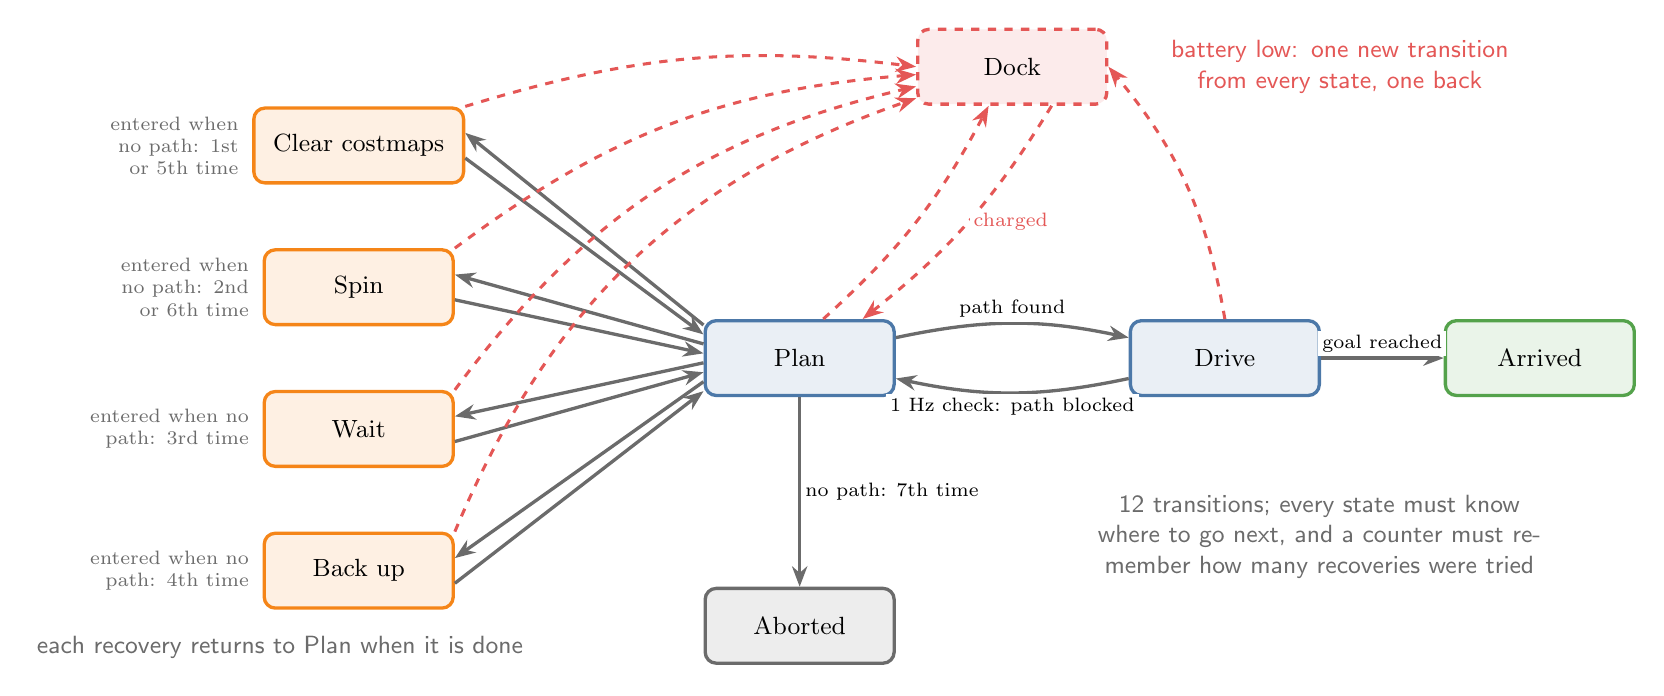
\begin{tikzpicture}[
  st/.style={box=#1, font=\small, minimum width=2.4cm, minimum height=0.95cm},
  lab/.style={font=\scriptsize, text=black, fill=white, inner sep=1.5pt},
  tr/.style={-{Stealth[length=2.6mm]}, draw=cgrey, line width=1.2pt},
  dock/.style={-{Stealth[length=2.6mm]}, draw=cred, line width=1.1pt, dashed}]
  \node[st=cblue] (plan) at (0,0) {Plan};
  \node[st=cblue] (drive) at (5.4,0) {Drive};
  \node[st=cgreen] (arr) at (9.4,0) {Arrived};
  \node[st=cgrey] (ab) at (0,-3.4) {Aborted};
  \node[st=cred, dashed] (dock) at (2.7,3.7) {Dock};
  \foreach \n/\t/\y/\c/\o in {clear/Clear costmaps/2.7/{1st or 5th}/3.6, spin/Spin/0.9/{2nd or 6th}/1.2,
                              wait/Wait/-0.9/3rd/-1.2, back/Back up/-2.7/4th/-3.6} {
    \node[st=corange] (\n) at (-5.6,\y) {\t};
    \node[lab, anchor=east, text=cgrey, text width=2.5cm, align=right] at ([xshift=-1mm]\n.west) {entered when no path: \c\ time};
    \draw[tr] ([yshift=\o mm+0.6mm]plan.west) -- ([yshift=1.6mm]\n.east);
    \draw[tr] ([yshift=-1.6mm]\n.east) -- ([yshift=\o mm-0.6mm]plan.west);
  }
  \draw[tr] (plan) to[bend left=12] node[lab, above] {path found} (drive);
  \draw[tr] (drive) to[bend left=12] node[lab, below] {1 Hz check: path blocked} (plan);
  \draw[tr] (drive) -- node[lab, above] {goal reached} (arr);
  \draw[tr] (plan) -- node[lab, right] {no path: 7th time} (ab);
  \node[note, anchor=north] at (-6.6,-3.4) {each recovery returns to Plan when it is done};
  % docking added
  \draw[dock] (drive.north) to[bend right=15] (dock.east);
  \draw[dock] ([xshift=3mm]plan.north) to[bend right=10] ([xshift=-3mm]dock.south);
  \draw[dock] (clear.north east) to[bend left=12] (dock.west);
  \draw[dock] (spin.north east) to[bend left=16] ([yshift=-1mm]dock.west);
  \draw[dock] (wait.north east) to[bend left=20] ([yshift=-2.5mm]dock.west);
  \draw[dock] (back.north east) to[bend left=24] ([yshift=-4mm]dock.west);
  \draw[dock] ([xshift=5mm]dock.south) to[bend left=10] node[lab, text=cred, right] {charged} ([xshift=8mm]plan.north);
  \node[note, text=cred, anchor=west, text width=4.6cm] at ([xshift=0.5cm]dock.east) {battery low: one new transition from every state, one back};
  \node[note, anchor=north, text width=6.6cm] at (6.6,-1.6) {12 transitions; every state must know where to go next, and a counter must remember how many recoveries were tried};
\end{tikzpicture}
\end{document}
